% !TeX encoding = UTF-8

\chapter{ANÁLISE DOS RESULTADOS}\label{ch:resultados}
Este capítulo tem como finalidade apresentar os resultados obtidos através das implementações demonstradas no Capítulo 5.

\section{ANÁLISE DAS SÉRIES UTILIZADAS}
Após a implementação do modelo da RNA, através dos conjuntos de dados coletados, faz-se necessário avaliar como a respectiva técnica se comportou. Tendo isso em vista, a mesma foi aplicada em função do objetivo principal do trabalho, que é medir a capacidade de precisão de acerto no valor de abertura das ações. Portanto, foi elaborada, de forma independente, uma análise de eficácia do modelo para o cenário de cada empresa utilizada no presente trabalho. É importante ressaltar que os modelos foram implementados levando em consideração todos os \textit{scripts}, métodos e ferramentas utilizadas no capítulo anterior.

\subsection{Aplicação da rede na Intel Corporation}
A rede da Intel Corporation foi treinada com o objetivo de capturar o maior nível de variação possível dos dados, visando mapear um maior conjunto de padrões e, assim, responder de forma eficiente à dados dispersos através de uma boa capacidade de generalização. Tendo isso em vista, o período de treinamento preparado foi de 09/04/2001 até 21/08/2017, totalizando 4117 registros.

Para o presente caso foram construídos dois cenários de simulação, buscando obter um parâmetro de ciclos de treinamento adequado ao modelo de dados utilizado. As métricas definidas para análise, a partir destes ciclos de treinamento, são: o comportamento da função de custo que compõem o modelo (erro quadrático médio, EQM) e a margem de erro dos valores resultantes da rede, no período de 23/08/2017 a 31/08/2017, em relação aos valores reais. Os parâmetros utilizados foram: 200 e 1000 iterações.

\subsubsection{Treinamento com 200 Iterações}	
A ideia de executar o treinamento com uma quantidade baixa de iterações, é feita com o intuito de proporcionar um treinamento mais rápido e com resultados significativos, levando em consideração as características especificas do modelo de dados. Portanto, para quantificar como ocorreu o processo de treinamento, basta multiplicar o número de iterações (200) com o número de registros de testes (4117), resultando em um total de 823.400 exemplos calculados pela rede. O Gráfico 8 demonstra, de acordo com a quantidade de ciclos, a variação do EQM no primeiro cenário de teste com 200 iterações.
\begin{grafico}[h]
	\centering
	\fbox{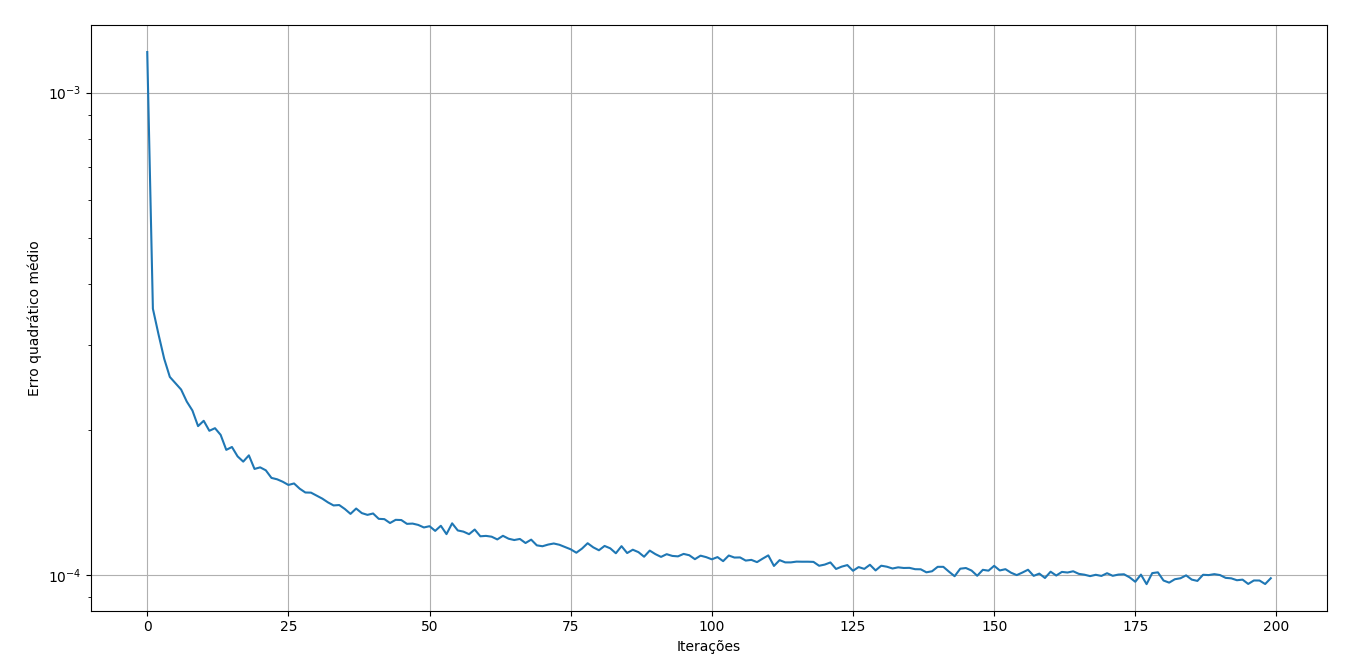
\includegraphics[width=1\textwidth]{erro_intel_primeiro}}
	\caption{Decaimento do EQM no treinamento da rede}
	\fonte{Elaborado pelo autor}
	\label{lingua}
\end{grafico}

O EQM iniciou-se, na primeira iteração, com um erro percentual de 0.00248996652176 e, após o término das 200 épocas de treinamento, conclui-se com um erro percentual de 9.49359025338.$10^{-05}$. Analisando o gráfico, pode-se observar que o erro obteve uma queda brusca nas primeiras 75 iterações, enquanto que, nas 125 iterações posteriores, manteve o padrão com valores aproximados. A queda brusca e rápida do valor está diretamente ligada a capacidade de aprendizado e adaptação ao modelo de dados.

Já o Gráfico 9 demonstra, de acordo com a quantidade de ciclos, a variação do EQM no segundo cenário de teste com 200 iterações.
\begin{grafico}[h]
	\centering
	\fbox{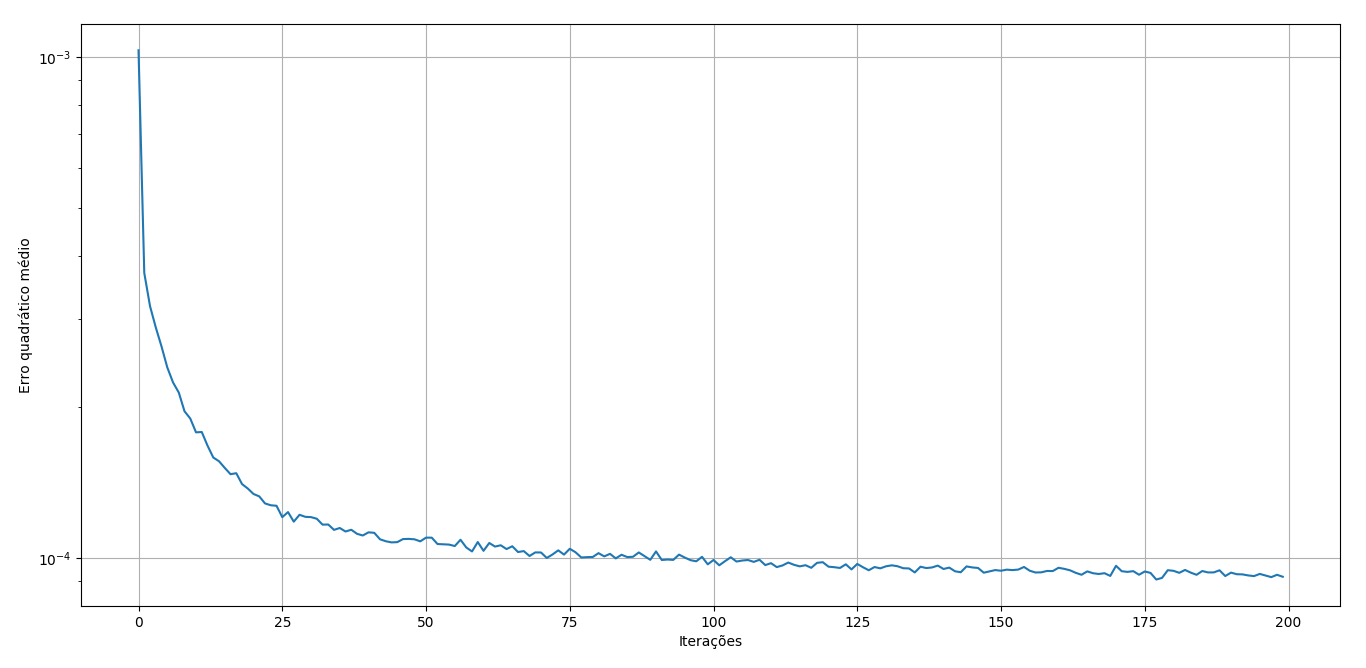
\includegraphics[width=1\textwidth]{erro_intel_segundo_cenario}}
	\caption{Decaimento do EQM no treinamento da rede}
	\fonte{Elaborado pelo autor}
	\label{lingua}
\end{grafico}

Neste cenário, o erro foi iniciado com um percentual de 0.00102981131422 e, após o término das 200 épocas de treinamento, concluí-se com um erro percentual de 9.1790170623e.$10^{-05}$. Analisando os Gráficos 8 e 9, pode-se observar que apesar da rede ser iniciada com os pesos aleatoriamente, o EQM seguiu a mesma tendência para os dois cenários, isso implica em uma confiabilidade maior por parte do algoritmo, pois o mesmo garante que novas inicializações, aplicadas ao mesmo modelo de dados, não resultam em erros muito distintos.

Após a verificação do comportamento do EQM, a rede foi exposta ao período de teste. Na Tabela 1 são detalhados os valores aplicados.
\begin{table}[h]
\centering
\caption{Período dos dados utilizados para testes: Intel Corporation}
\vspace{0.5cm}
\begin{tabular}{>{\centering\arraybackslash}m{2cm} >{\centering\arraybackslash}m{2cm} >{\centering\arraybackslash}m{2cm} >{\centering\arraybackslash}m{2cm} >{\centering\arraybackslash}m{2cm} >{\centering\arraybackslash}m{2cm}}
\toprule
Data    & Abertura   & Alta   & Baixa   & Fechamento   & Volume\\
\midrule
23/08/2017 & 34.54 & 34.81 & 34.38 & 34.66 & 196.481,34\\
24/08/2017 & 34.70 & 34.89 & 34.55 & 34.71 & 143.018,92\\
25/08/2017 & 34.82 & 34.93 & 34.58 & 34.67 & 147.268,29\\
28/08/2017 & 34.78 & 34.80 & 34.59 & 34.65 & 207.128,76\\
29/08/2017 & 34.51 & 34.75 & 34.46 & 34.73 & 158.436,68\\
30/08/2017 & 34.75 & 34.96 & 34.63 & 34.89 & 185.650,07\\
31/08/2017 & 34.94 & 35.18 & 34.87 & 35.07 & 163.667,72\\
\bottomrule
\end{tabular}
\end{table}

Os dados demonstrados na Tabela 1 foram refinados e normalizados de acordo com os métodos implementados no Capítulo 5. Após a execução deste processo, os mesmos foram inseridos na RNA para ativação. Posteriormente, foi realizada a desnormalização e os resultados apresentados. A Tabela 2 ilustra os resultados obtidos.
\begin{table}[h]
\centering
\caption{Resultados da predição realizada nos dados utilizados pela rede}
\vspace{0.5cm}
\begin{tabular}{>{\centering\arraybackslash}m{3cm} >{\centering\arraybackslash}m{3cm} >{\centering\arraybackslash}m{3cm} >{\centering\arraybackslash}m{3cm}}
\toprule
Data    & Valor esperado   & Resultado    & Erro (\%)\\
\midrule
23/08/2017 & 34.54 & 34.73 & 0.550\\
24/08/2017 & 34.70 & 34.71 & 0.028\\
25/08/2017 & 34.82 & 34.79 & 0.086\\
28/08/2017 & 34.78 & 34.77 & 0.028\\
29/08/2017 & 34.51 & 34.75 & 0.695\\
30/08/2017 & 34.75 & 34.82 & 0.201\\
31/08/2017 & 34.94 & 34.99 & 0.143\\
\bottomrule
\end{tabular}
\end{table}

Analisando a Tabela 2, pode-se observar que os resultados obtidos foram significativos, onde o percentual de erro calculado, através do erro relativo percentual, não ultrapassou a margem 0.70\%, se aproximando, consideravelmente, dos valores reais. O erro médio, analisado para todo o período de predição, ficou em torno de 0.20\%, o que pode ser considerado baixo levando-se em conta o número de iterações utilizadas para treinar a RNA. O Gráfico 9 representa, de maneira ilustrativa, os resultados da série.
\begin{grafico}[h]
	\centering
	\fbox{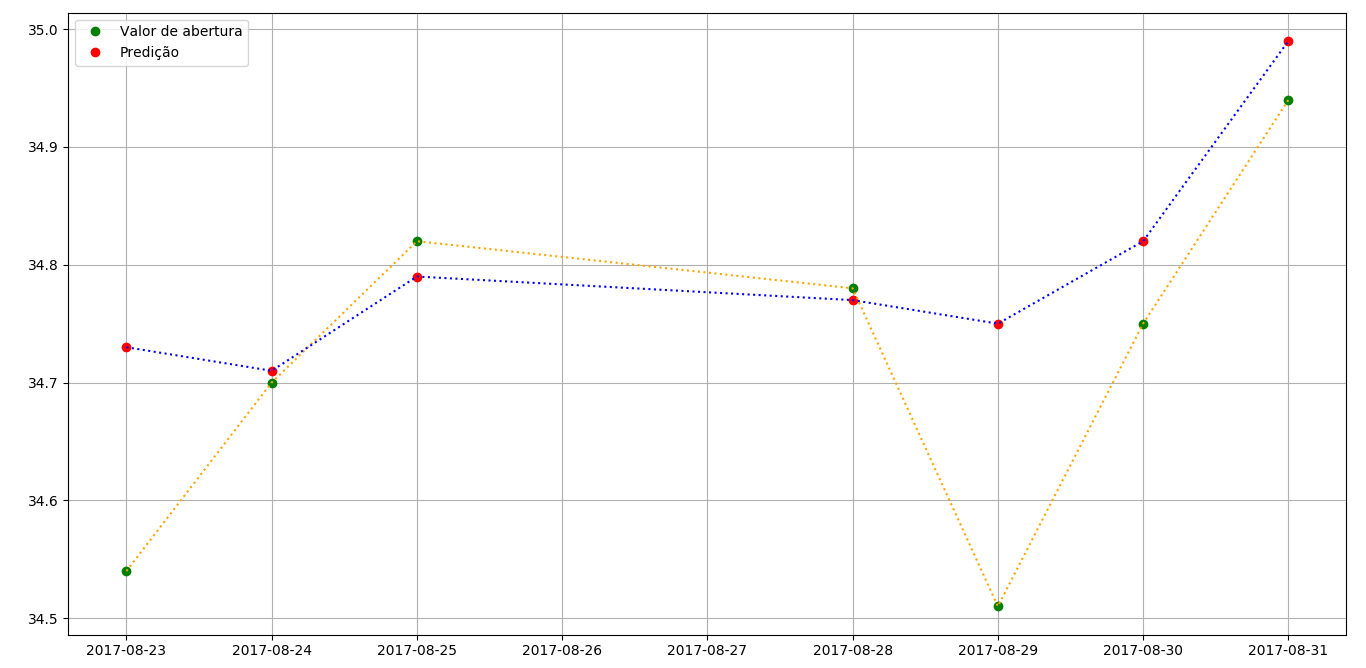
\includegraphics[width=1\textwidth]{predicao_intel}}
	\caption{Distribuição dos dados resultantes da RNA e seus valores esperados}
	\fonte{Elaborado pelo autor}
	\label{lingua}
\end{grafico}

Pelo gráfico também é possível observar como os resultados são próximos aos esperados. Os valores de abertura, nos respectivos dias testados, são representados por um ponto verde. Já os resultados obtidos pela rede são caracterizados pelo ponto vermelho. 

\subsubsection{Treinamento com 1000 Iterações}	
Para comparar com a simulação anterior foi realizado um teste com 1000 épocas de treinamento, visando alcançar um resultado mais preciso e, também, validar se o aumento na quantidade de iterações, no processo de treinamento, melhoram os resultados retornados pela rede.

Para quantificar como ocorreu o processo de treinamento, basta multiplicar o número de iterações (1000) com o número de registros de testes (4117), resultando em um total de 4.117.000 exemplos calculados pela rede.
\begin{grafico}[h]
	\centering
	\fbox{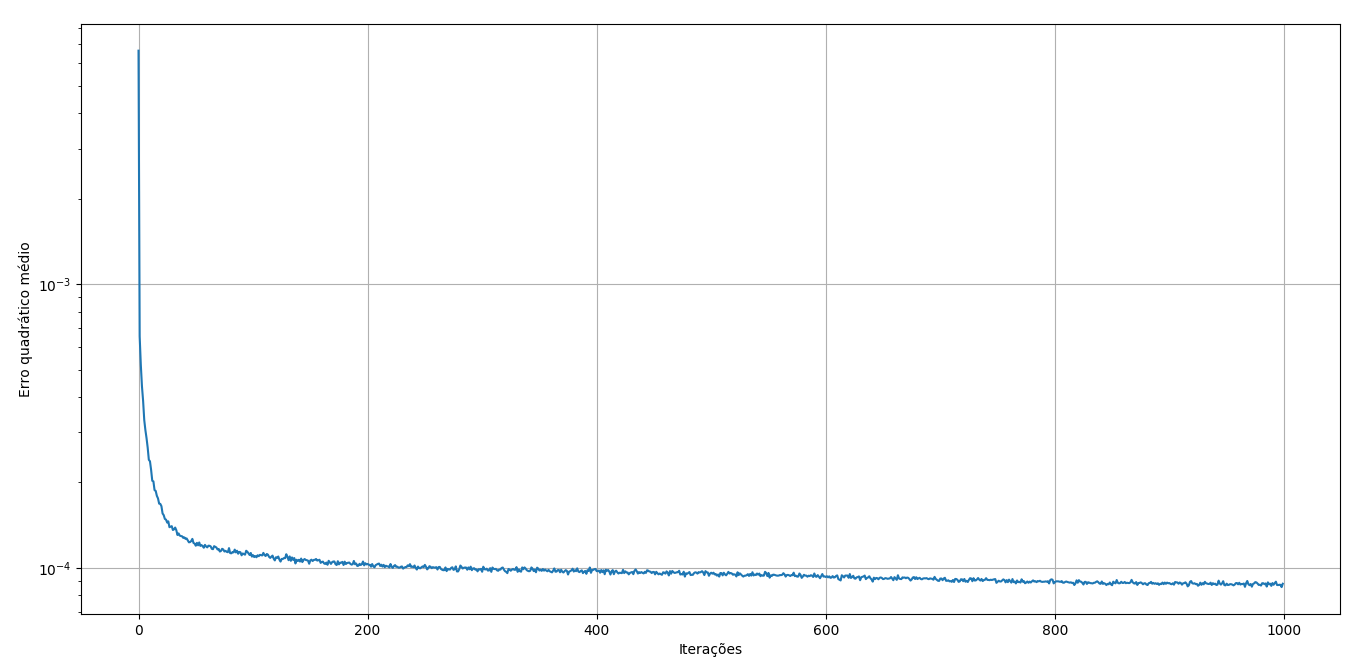
\includegraphics[width=1\textwidth]{erro_intel_1000iteracoes}}
	\caption{Decaimento do EQM no treinamento da rede}
	\fonte{Elaborado pelo autor}
	\label{lingua}
\end{grafico}

Para este cenário a rede iniciou-se, na primeira iteração, com um erro percentual de 0.00664064049629 e, após o término das 1000 épocas de treinamento, conclui-se com um erro percentual de 8.7943563121853531.$10^{-05}$. 

Analisando o Gráfico 11, pode-se observar que o erro obteve uma queda constante até 200 iterações, enquanto que, entre as iterações de número 200 até a de número 400, manteve o padrão com valores aproximados. Os últimos 600 ciclos mantiveram um decaimento mínimo do EQM.

Tendo em vista a simulação anterior, fica claro que a queda brusca e rápida aconteceria, pois a base de dados utilizada é a mesma, mas com um número maior de iterações, fazendo com que o EQM obtenha resultados mais baixos em comparação ao treino anterior.

O período para realizar os testes foi o mesmo utilizado na Tabela 1. Os dados foram devidamente refinados e normalizados e, a partir disto, foram ativados na rede. Os resultados obtidos são demonstrados na Tabela 3.
\begin{table}[h]
\centering
\caption{Resultados da predição realizada nos dados utilizados pela rede}
\vspace{0.5cm}
\begin{tabular}{>{\centering\arraybackslash}m{3cm} >{\centering\arraybackslash}m{3cm} >{\centering\arraybackslash}m{3cm} >{\centering\arraybackslash}m{3cm}}
\toprule
Data    & Valor esperado   & Resultado    & Erro (\%)\\
\midrule
23/08/2017 & 34.54 & 34.67 & 0.376\\
24/08/2017 & 34.70 & 34.64 & 0.172\\
25/08/2017 & 34.82 & 34.71 & 0.315\\
28/08/2017 & 34.78 & 34.68 & 0.287\\
29/08/2017 & 34.51 & 34.65 & 0.405\\
30/08/2017 & 34.75 & 34.70 & 0.143\\
31/08/2017 & 34.94 & 34.84 & 0.286\\
\bottomrule
\end{tabular}
\end{table}

Analisando a Tabela 3, pode-se observar que os resultados obtidos foram significativos, onde o percentual de erro calculado, através do erro relativo percentual, não ultrapassou a margem 0.50\%, se aproximando consideravelmente dos valores reais. Porém, a média de todo o período analisado obteve um erro de 0.28\%, superior ao treinamento anterior. O Gráfico 12 representa, de maneira ilustrativa, os resultados da série.
\begin{grafico}[h]
	\centering
	\fbox{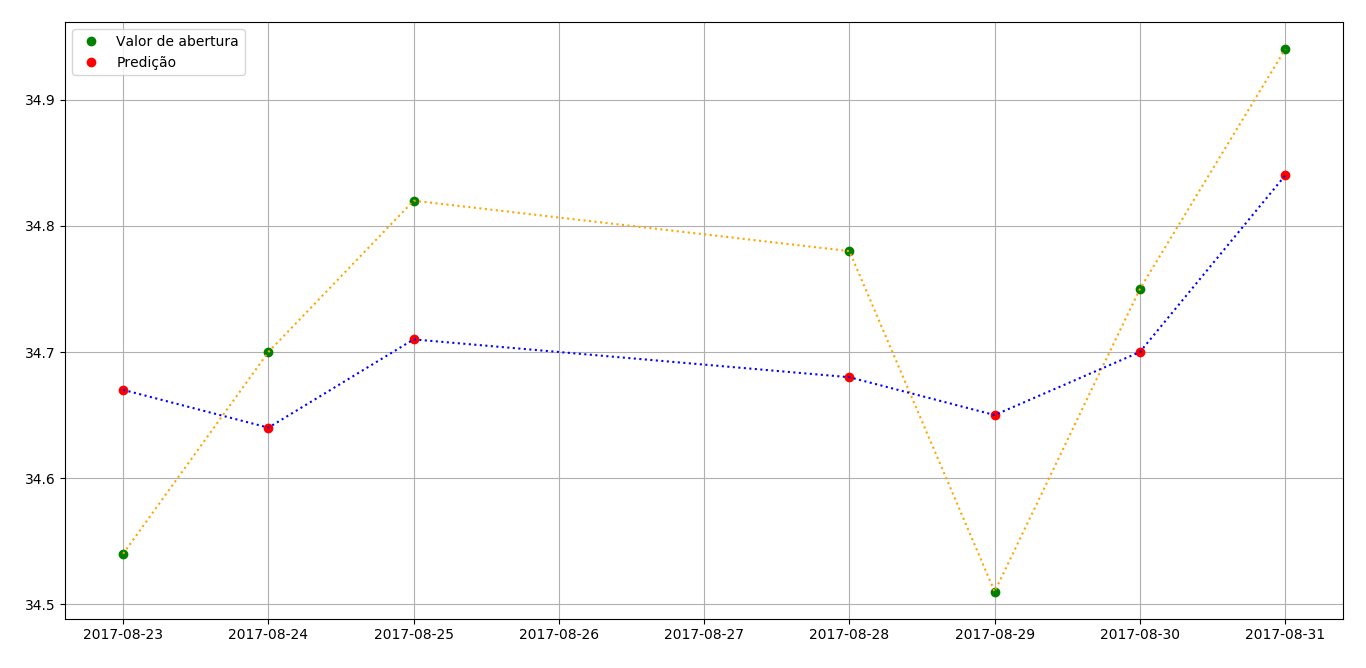
\includegraphics[width=1\textwidth]{predicao_intel_1000}}
	\caption{Distribuição dos dados resultantes da RNA e seus valores esperados}
	\fonte{Elaborado pelo autor}
	\label{lingua}
\end{grafico}

Apesar da diferença do erro percentual relativo entre os dois cenários ser de apenas 8\%, foi encontrada uma melhor parâmetrização para o presente modelo de dados utilizado em 200 iterações. Sendo assim, chega-se a definição que nem sempre um número maior de ciclos de treinamento aumentam a precisão da RNA. Neste caso, a rede sofreu uma convergência do EQM em torno de 200 iteraçoes, este detalhe pode ser observado visualizando o comportamento dos Gráficos 8 e 10. Dessa forma, as iterações posteriores propagaram o erro de forma desnecessária, alterando assim os pesos sinápticos dos neurônios e, automaticamente, causando uma maior dispersão nos resultados. Este processo ocorrido na segunda simulação, na literatura, é denominado \textit{Overtraining}, detalhado no Capítulo 3.